\documentclass[10pt]{article}
\usepackage[a4paper, total={7in,10in}]{geometry}
\usepackage{hyperref}
\usepackage{siunitx}
\usepackage{graphicx}
\usepackage{caption}
\usepackage[backend=biber]{biblatex}
\addbibresource{report.bib}

%opening
\title{EP2420 Project 2 - Forecasting Service Metrics}
\author{André Silva}
\begin{document}

\maketitle

\section*{Task II}
\label{sec:2}

In this task we use a Recurrent Neural Network (RNN)~\cite{RNN} to predict, not the current state of a service metric, but the future states of said metric. 

More specifically, we will be using a Long Short-Term Memory (LSTM) Network~\cite{LSTM}.
LSTM is a RNN architecture that mitigates the vanishing gradient problem by introducing $3$ gates and a memory cell per unit. This allows each unit to model the remembrance and addition of, respectively, old and new memory. Being a RNN architecture, it also allows us to process, not only but also, sequences of data and build models that take into account the order embedded in sequences.

First, we pre-process the trace, standardizing along each column and removing outliers that deviate more than $40\sigma$. We also apply tree-based feature selection, using 10 estimators, to get the top $16$ features.

After this, we split the trace into training and test sets, and then transform them into new datasets that follow the structure $([x^{(t-l)},...,x^{(t)}],[y^{(t)},...,y^{(t+h)}])$. As we are using analyzing \textit{KV periodic}~\cite{9012741}, our step size (i.e. time between each sample of a sequence), is $1$ second.

We then perform an experiment to study the impact of $l$ on the accuracy of a model and its predictions of $0...10$ steps into the future by building $11$ different models with $l\in\{0,...,10\}$. In this experiment we build stacked LSTM Networks~\cite{SLSTM}, composed of 3 layers. The first layer is an LSTM layer with $100$ units, the second layer is an LSTM layer with $50$ units, while the third and final layer is a Dense layer with $h+1$ units, corresponding to the output. Each model was trained for $100$ epochs, using \texttt{Adam} as the optimization algorithm and the mean-squared error as the loss function. The default values were utilized for all other parameters.

The results can be found below in Figure $\ref{fig:2}$.

\begin{figure}[h!]
    \centering
    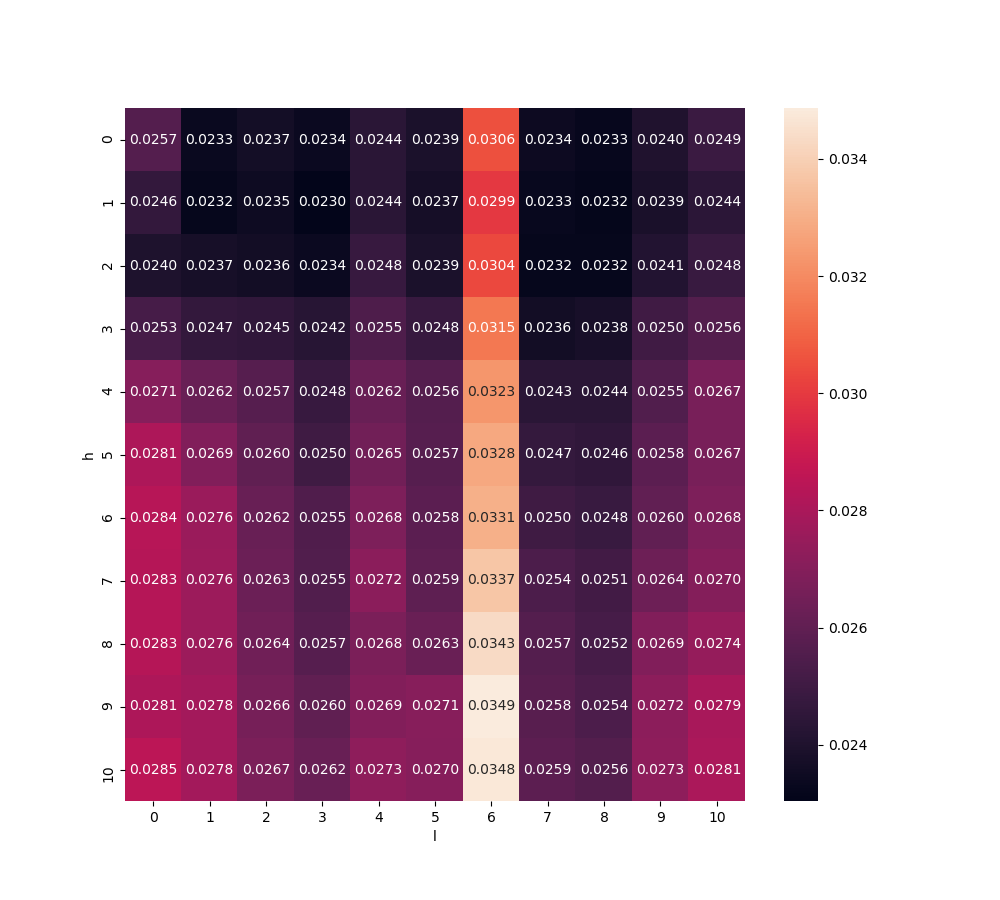
\includegraphics[width=0.65\textwidth,height=\textheight,keepaspectratio]{../result/project2/lstm_nmae_heatmap.png}
    \caption{Heat-map of \textsc{NMAE} for each stacked LSTM~\cite{SLSTM} model with $l\in\{0,...,10\}$ when predicting $y^{(t+h)}$}
    \label{fig:2}
\end{figure}


Figure \ref{fig:2} shows us the \textsc{NMAE} of each model when predicting $y^{(t+h)}$. Rows represent the time horizon $h = 0,...,10$ and columns represent the lag $l = 0,...,10$. The color gradient of the heat-map allows us to visualize and extract conclusions better than if we used a normal table.

When we analyze the results by looking at each row we notice that, in most cases, the \textsc{NMAE} decreases as we increase $l$. On the other hand, when we look at each column, we see that the \textsc{NMAE} increases as we increase $h$. Both these events are, intuitively, expected. When we increase $l$, we are providing more information, or context, to the model, so we expect better predictions. When we increase $h$, we are asking for a value that is more distant in time, and so, harder to predict.

This being said, we can clearly see that the model for $l = 6$ presents very deviated results. This could suggest that, during the training phase, the model hit a local optima or it is overfit, not allowing it to reach the same level of accuracy as the other models.

We can also see that, as in Task I, the \textsc{NMAE} doesn't monotonically decrease as we increase $l$ from 0, as expected. One possible explanation, other than the two, still applicable, explanations suggested in the previous Task, could be related to the training of each model, seeing that each model converges differently.

When comparing these results with the results of Task I, we notice that, in most cases, our \textsc{NMAE}s are lower, which could be explained by the fact that Neural Networks can, theoretically, approximate any given function, which is not the case for Linear Regression.
We can also see that the gradient of the results along the $h$ axis is lower, suggesting that these models can also better forecast than the previous one.

\printbibliography

\end{document}
